\subsubsection{Listar}

  \paragraph{}Para mostrar esta lista, es necesario establecer el centro para
  el que mostrar las asignaturas disponibles. Para ello, habrá que elegir el
  centro en la lista desplegable que se muestra en la figura
  \ref{capturaPantallaSelectCentro}.

  \paragraph{}También será necesario elegir la titulación a la que pertenecen
  las asignaturas, por lo que se elegirá entre las opciones de una lista
  desplegable, siguiendo el mismo mecanismo que para seleccionar centro. Se
  puede ver una captura de la selección de titulación en la figura
  \ref{capturaPantallaSelectTitulacion}.

  \begin{figure}[!ht]
    \begin{center}
      \fbox{
      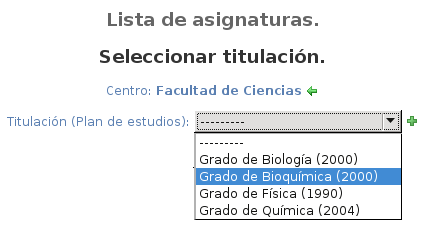
\includegraphics[scale=0.55]{4.Funcionamiento_Aplicacion/4.3.Gestion/4.3.1.Administrador_Principal/4.3.1.6.Asignatura/select_titulacion.png}
      }
      \caption{Captura de pantalla de la lista desplegable para seleccionar titulación para el usuario \textit{Administrador principal}.}
      \label{capturaPantallaSelectTitulacion}
    \end{center}
  \end{figure}

  \paragraph{}Nótese que si no existieran elementos disponibles en el sistema,
  la lista desplegable aparecería vacía. Por tanto, se proporciona al usuario
  un icono, representado por una cruz verde, para añadir nuevos elementos al
  sistema. Este icono es el mostrado en la figura \ref{capturaBotonAdd}. Al
  pulsar dicho botón, aparecerá la ventana de creación de un nuevo elemento.

  \paragraph{}Una vez seleccionados el centro y la titulación, se muestra la
  lista completa de asignaturas que aparecen en el sistema. La figura
  \ref{capturaPantallaListaAsignaturasAdminPrincipal} muestra
  una captura de pantalla de la lista de asignaturas.

  \begin{figure}[!ht]
    \begin{center}
      \fbox{
      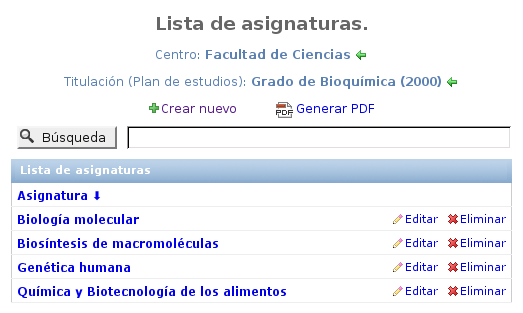
\includegraphics[scale=0.55]{4.Funcionamiento_Aplicacion/4.3.Gestion/4.3.1.Administrador_Principal/4.3.1.6.Asignatura/lista_asignaturas.png}
      }
      \caption{Captura de pantalla de la lista de asignaturas para el usuario \textit{Administrador principal}.}
      \label{capturaPantallaListaAsignaturasAdminPrincipal}
    \end{center}
  \end{figure}

  \paragraph{}Si se quisiera refinar el listado de elementos mostrados, es
  posible seleccionar nuevos parámetros pulsando el icono \textit{Seleccionar}
  que aparece al lado de cada elemento. Este icono aparece en la figura
  \ref{capturaBotonSeleccionar}.
